\documentclass[../../thesis.tex]{subfiles}

\graphicspath{{./img/}}



\begin{document}


\section{Motifs in Temporal Networks}
\label{sec:motifs_temporal_network}

Temporal network motifs are induced subgraphs on sequences of temporal edges, as is definedion the work of \citeauthor{temporalMotifs}. It is based on generalizing the concept of static network motifs towards temporal networks\cite{temporalMotifs}.  Before we continue our study, we must first define the vocabulary used by \citeauthor{temporalMotifs}.


\subsection{Definitions}
\label{sec:motifs_definitions}

 

\theoremstyle{definition}

\theoremstyle{definition}
\begin{definition}{\textbf{Temporal Edges:}}
A timestamped directed edge between an ordered pair of nodes (a line from the Table~\ref{fig:inputSolutionTableGraphA}). Formally, given a node set \textit{V}, a tuple \textit{($u_{i}$, $v_{i}$, $t_{i}$), i = 1,...,m}, is a temporal edge if \textit{$u_{i}$} and \textit{$v_{i}$} are elements of \textit{V} and \textit{$t_{i}$} is a timestamp in $\mathbb{R}$. There can be many temporal edges directed from \textit{u} to \textit{v}, and we refer to them as edges between \textit{u} and \textit{v}. We assume that the timestamps $t_{i}$ are unique.
\end{definition}
\label{def:temporal_edge}



\theoremstyle{definition}
\begin{definition}{\textbf{Temporal Graph:}}
A collection of temporal edges (Fig. \ref{fig:inputSolutionTableGraphB}, Fig. \ref{fig:intro1A}). Formally, a temporal graph \textit{T} on a node set \textit{V} is a collection of tuples \textit{($u_{i}$, $v_{i}$, $t_{i}$), i = 1,...,m}, where each \textit{$u_{i}$} and \textit{$v_{i}$} are elements of \textit{V} and each \textit{$t_{i}$} is a timestamp in $\mathbb{R}$.

\end{definition}
\label{def:temporal_graph}

\begin{definition}{\textbf{$\delta$-Temporal Motifs:}}
Classes of isomorphic subgraphs (Fig. \ref{fig:intro1B}) where it takes into account the ordering of edges.
\end{definition}
\label{def:delta_temporal_motif}

\theoremstyle{definition}
\begin{definition}{\textbf{Instance of $\delta$-Temporal Motif:}}
A collection of edges in a given temporal graph is an instance of a $\delta$-temporal motif \textit{M} that matches the same edge pattern and all of the edges occur in the right order within the time window (Fig. \ref{fig:intro1C}). Properly, any time-ordered sequence \textit{S = ($w_{1}$, $x_{1}$, $t_{1}'$),..., ($w_{l}$, $x_{l}$, $t_{l}'$)} of \textit{l} unique edges is an instance of the motif \textit{M = ($u_{1}$, $v_{1}$, $t_{1}$), ..., ($u_{l}$, $v_{l}$, $t_{l}$)} if:
\begin{enumerate}
  \item {There exists a bijection \textit{f} on the vertices such that \textit{$f(w_{i}) = u_{i}$} and $f(x_{i})=v_{i}$, i = 1,...,l;}
  \item {All the edges occur within  $\delta$ time, i.e., $t_{l}' - t_{1}' \leq \delta$;}
\end{enumerate}

\end{definition}
\label{def:instance_delta_temporal_motif}



\theoremstyle{definition}
\begin{definition}{\textbf{Induced Static Graph:}}
Finally, by ignoring timestamps and duplicate edges, the temporal graph induces a standard directed graph, which we call the static graph \textit{G} of \textit{T} with static edges, i.e., \textit{(u, v)} is an edge in \textit{G} if and only if there is some temporal edge \textit{(u, v, t)} in \textit{T}. 

\end{definition}
\label{def:induced_static_graph}

\begin{figure}[H]
\centering
% Put these subfigures here to get cross referencing (HACK)
\begin{subfigure}[b]{0.3\textwidth}\phantomcaption\label{fig:intro1A}\end{subfigure}
\begin{subfigure}[b]{0.3\textwidth}\phantomcaption\label{fig:intro1B}\end{subfigure}
\begin{subfigure}[b]{0.3\textwidth}\phantomcaption\label{fig:intro1C}\end{subfigure}
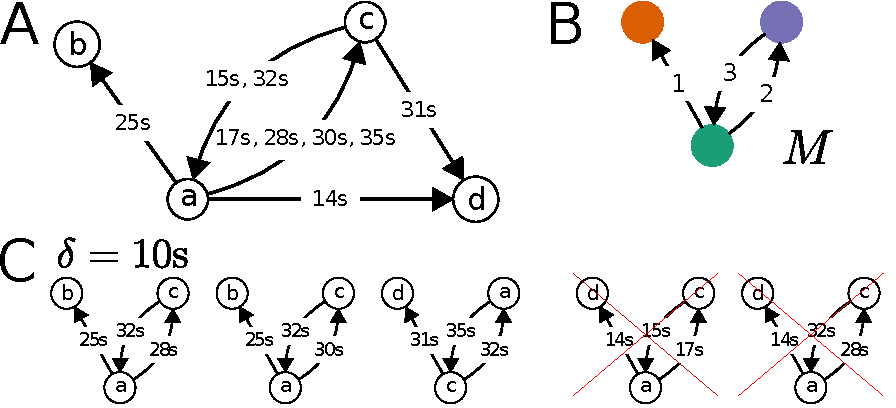
\includegraphics[width=\columnwidth]{content/unveiling/img/intro1}
\caption{%
\textnormal{A}) A temporal graph with nine temporal edges.  Each edge
has a timestamp (listed here in seconds).
%
\textnormal{B}) Example of a $3$-node, $3$-edge $\delta$-temporal motif $M$.  The
edge labels correspond to the ordering of the edges.
%
\textnormal{C})
Instances of the $\delta$-temporal motif $M$ in the graph for $\delta$ = 10
seconds.  The crossed-out patterns are not instances of $M$ because either the
edge sequence is out of order or the edges do not all occur within the time
window $\delta$.
%
\vspace{-0.7cm}
}
\label{fig:intro1}
\end{figure}

\subsection{Counting Temporal Motifs}
\label{sec:motifs_couting}


The work of \citeauthor{temporalMotifs} describes a general algorithm for the problem of counting how many times each $\delta$-temporal motif occurs in a given temporal network. The central goal is to count the number of ordered length-\textit{l} of edges that are instances of a given \textit{k}-node, \textit{l}-edge, $\delta$-temporal motif, from a given temporal graph \textit{T}.  Even though the proposed algorithm is a general approach, we are only interested in small patterns. 


The mentioned algorithm for counting instances of temporal motifs in a temporal graph \textit{T} has as \textit{Input}: Sequence \textit{S'} of edges \textit{($u_{1}$, $v_{1}$, $t_{1}$),...,($u_{L}$, $v_{L}$, $t_{L}$)} with \textit{$t_{1}<...<t_{L}$}, time window  $\delta$ and as \textit{Output}: A $6X6$ matrix storing the number of instances of each 2-node and 3-node, 3-edge $\delta$-temporal motifs contained in the sequence. Figure~\ref{fig:all_three_edge_motifs} provides a visualization of all motifs from the 6X6 matrix output.

The algorithm can assess the count respecting different types of motifs: 2-node, stars, and triangles. Furthermore, the algorithm is divided into three procedures which evaluates each kind of motif. The algorithm starts with a \textit{general approach} that follows the above steps:
\begin{enumerate}
  \item{Identify all instances \textit{$H'$} of the static motif \textit{H} induced by \textit{M} within the static graph \textit{G} induced by the temporal graph \textit{T}.}
  \item{For each static motif instance \textit{$H'$}, gather all temporal edges between pairs of nodes forming an edge in \textit{$H'$} into an ordered sequence \textit{$S'=(u_{1}$, $v_{1}$, $t_{1}$),...,($u_{L}$, $v_{L}$, $t_{L}$)}}  
  \item{Count the number of subsequences of edges in \textit{$S'$} occurring within delta time units that correspond to instances of \textit{M}. }
\end{enumerate}


Any induced graph \textit{H} of a 2-node  $\delta$-temporal motif is either a single or a bidirectional edge. Then, if the motif is of type 2-node motifs, the algorithm runs those steps:
\begin{enumerate}
  \item{For each pair of nodes \textit{u} and \textit{v} for which there is at least one edge, gather and sort the edges in either direction between \textit{u} and \textit{v};}
  \item{Call the above general approach with these edges;}
  \item{Then, sum all the returns of (2) to obtain the total motif count.}
\end{enumerate}

However, if the type of the \textit{k}-node, \textit{l}-edge motif is a star type, the induced static graph \textit{H} consists of a center node and $k-1$ neighbors, where edges may occur in either direction between the center node and a neighbor node. Then, the algorithm use this information to computes the following steps:
\begin{enumerate}
  \item{For each node \textit{u} in the static graph and for each unique set of $k-1$ neighbors, gather and sort the edges in either direction between \textit{u} and the neighbors;}
  \item{Call the general approach with these edges;}
  \item{Each return counts from (2) are summed across all center nodes.}
\end{enumerate}


Finally, in triangle motifs types, the induced graph \textit{H} consists of 3 nodes and at least one directed edge between any pair of nodes. The induced static graph \textit{H} of \textit{M} contains at least three and at most six static edges. 
Thus, if the type of the motif is a triangle, the algorithm evaluates those steps:
\begin{enumerate}
  \item{Use the algorithm proposed by \cite{latapy2008main_14} to find all triangles in the static graph \textit{G} induced by \textit{T};}
  \item{For each triangle \textit{$(u, v, w)$}, merge all temporal edges from each pair of nodes to get a time-sorted list of edges;}
  \item{Use general approach to count the number of instances of \textit{M}.}
\end{enumerate}


These methods are able to count the number of instances of any \textit{k}-node, \textit{l}-edge $\delta$-temporal motif. However, this method is only optimal for 2-node and 3-node motifs, and the computational cost may be expensive for other motif types. Consequently, the output of the algorithm only counts instances of 2-node and 3-node, 3-edge delta-temporal motifs. For more details of the algorithm, see \cite{temporalMotifs}.



\begin{figure}[H]
\centering
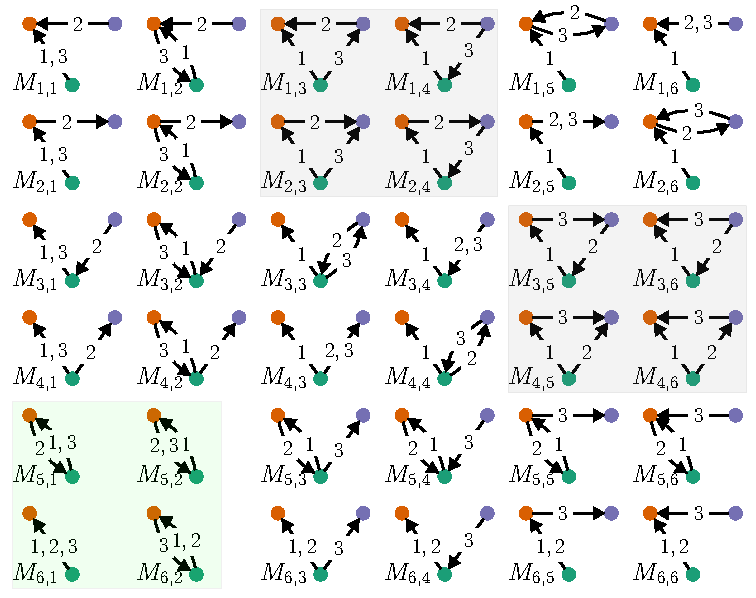
\includegraphics[width=0.8\textwidth]{content/unveiling/img/embedded-three-edge-all}
\caption{The output of the algorithm proposed above: A matrix with all $2$-node and $3$-node, $3$-edge $\delta$-temporal motifs counts. The 24 white background motifs are stars. The green background highlights the four $2$-node motifs (bottom left) and the grey background highlights the eight triangles. All the 36 motifs are indexed $M_{i,j}$ by 6 rows and 6 columns. The first edge in each motif is from the green to the orange node. The second edge is the same along each row, and the third edge is the same along each column.}
\label{fig:all_three_edge_motifs}
\end{figure}

What is exciting for us from the results achieved by \cite{temporalMotifs} was, applying the motif counting algorithm in a variety of temporal network datasets they were able to find that the number of instances of different $\delta$-temporal motifs reveals fundamental mechanisms of the networks. The algorithm was applied on a variety of datasets: a collection of emails between members of a European research institution, telephone call records for a major European service provider, a group of posts from StackOverflow, all the payments made up to October 19, 2014 from the Bitcoin Blockchain, and four more different datasets. 

They calculate the median time for a node to become part of three edges in the dataset to discover the most suitable delta time window to run the algorithm. Their results show $\delta=1$ hour for the time window. An empirical observation of the motif counts was made to examine the distribution of 2-node and 3-node, 3-edge motif instance counts from the target datasets. Two collections of datasets from similar domains were formed. The counts of the 36 different motifs were normalized to build the count distributions. As a result of those distributions, they conclude that temporal networks from the same domain have similar counts. This result confirms their motivation, where it resembles the results from \cite{milo2004superfamilies_18, vazquez2004topological_25, yaverouglu2014revealing_29}, static graphs from related domains tend to have similar motif count distributions.

\end{document}